%%%%%%%%%%%%%%%%%%%%%%%%%%%%%%%%%%%%%%%%%%%%%%%%%%%%%%%%%%%%%%%%%%%%%%%%
%%%%%%%%%%%%%%%%%%%%%% Simple LaTeX CV Template %%%%%%%%%%%%%%%%%%%%%%%%
%%%%%%%%%%%%%%%%%%%%%%%%%%%%%%%%%%%%%%%%%%%%%%%%%%%%%%%%%%%%%%%%%%%%%%%%

%%%%%%%%%%%%%%%%%%%%%%%%%%%%%%%%%%%%%%%%%%%%%%%%%%%%%%%%%%%%%%%%%%%%%%%%
%% NOTE: If you find that it says                                     %%
%%                                                                    %%
%%                           1 of ??                                  %%
%%                                                                    %%
%% at the bottom of your first page, this means that the AUX file     %%
%% was not available when you ran LaTeX on this source. Simply RERUN  %%
%% LaTeX to get the ``??'' replaced with the number of the last page  %%
%% of the document. The AUX file will be generated on the first run   %%
%% of LaTeX and used on the second run to fill in all of the          %%
%% references.                                                        %%
%%%%%%%%%%%%%%%%%%%%%%%%%%%%%%%%%%%%%%%%%%%%%%%%%%%%%%%%%%%%%%%%%%%%%%%%

%%%%%%%%%%%%%%%%%%%%%%%%%%%% Document Setup %%%%%%%%%%%%%%%%%%%%%%%%%%%%

% Don't like 10pt? Try 11pt or 12pt
\documentclass[10pt]{article}
\RequirePackage[T1]{fontenc}

% LaTeX will typeset using Computer Modern Roman, which a lot of
% non-mathematicians and non-engineers won't like. Also, a few PDF
% viewers may not render CMR very well. Instead, Times New Roman can
% be used. That's what this package does.
% \usepackage{times}

% The automated optical recognition software used to digitize resume
% information works best with fonts that do not have serifs. This
% command uses a sans serif font throughout. Uncomment both lines (or at
% least the second) to restore a Roman font (i.e., a font with serifs).
% (NOTE: This requires the times package above)
% \renewcommand{\familydefault}{\sfdefault}

% This is a helpful package that puts math inside length specifications
\usepackage{calc}
\usepackage{graphicx}
\usepackage{float}
% This package helps LaTeX auto-hyphenate hyphenated words if you use
% special hyphens. For example, bio\-/mimicry will properly hyphenate
% ``mimicry'' if necessary.
\usepackage[shortcuts]{extdash}

% Layout: Puts the section titles on left side of page
\reversemarginpar

%
%         PAPER SIZE, PAGE NUMBER, AND DOCUMENT LAYOUT NOTES:
%
% The next \usepackage line changes the layout for CV style section
% headings as marginal notes. It also sets up the paper size as either
% letter or A4. By default, letter was used. If A4 paper is desired,
% comment out the letterpaper lines and uncomment the a4paper lines.
%
% As you can see, the margin widths and section title widths can be
% easily adjusted.
%
% ALSO: Notice that the includefoot option can be commented OUT in order
% to put the PAGE NUMBER *IN* the bottom margin. This will make the
% effective text area larger.
%
% IF YOU WISH TO REMOVE THE ``of LASTPAGE'' next to each page number,
% see the note about the +LP and -LP lines below. Comment out the +LP
% and uncomment the -LP.
%
% IF YOU WISH TO REMOVE PAGE NUMBERS, be sure that the includefoot line
% is uncommented and ALSO uncomment the \pagestyle{empty} a few lines
% below.
%

%% Use these lines for letter-sized paper
\usepackage[paper=letterpaper,
            %includefoot, % Uncomment to put page number above margin
            marginparwidth=1.2in,     % Length of section titles
            marginparsep=.05in,       % Space between titles and text
            margin=1in,               % 1 inch margins
            includemp]{geometry}

%% Use these lines for A4-sized paper
%\usepackage[paper=a4paper,
%            %includefoot, % Uncomment to put page number above margin
%            marginparwidth=30.5mm,    % Length of section titles
%            marginparsep=1.5mm,       % Space between titles and text
%            margin=25mm,              % 25mm margins
%            includemp]{geometry}

%% More layout: Get rid of indenting throughout entire document
\setlength{\parindent}{0in}

% Provides special list environments and macros to create new ones
\usepackage[shortlabels]{enumitem}

%for text in the math equation
\usepackage{amsmath}
% Simpler bibsections for CV sections
% (thanks to natbib for inspiration)
%
% * For lists of references with hanging indents and no numbers:
%
%   \begin{bibsection}
%       \item ...
%   \end{bibsection}
%
% * For numbered lists of references (with hanging indents):
%
%   \begin{bibenum}
%       \item ...
%   \end{bibenum}
%
%   Note that bibenum numbers continuously throughout. To reset the
%   counter, use
%
%   \restartlist{bibenum}
%
%   at the place where you want the numbering to reset.

\makeatletter
\newlength{\bibhang}
\setlength{\bibhang}{1em}
\newlength{\bibsep}
 {\@listi \global\bibsep\itemsep \global\advance\bibsep by\parsep}
\newlist{bibsection}{itemize}{3}
\setlist[bibsection]{label=,leftmargin=\bibhang,%
        itemindent=-\bibhang,
        itemsep=\bibsep,parsep=\z@,partopsep=0pt,
        topsep=0pt}
\newlist{bibenum}{enumerate}{3}
\setlist[bibenum]{label=[\arabic*],resume,leftmargin={\bibhang+\widthof{[999]}},%
        itemindent=-\bibhang,
        itemsep=\bibsep,parsep=\z@,partopsep=0pt,
        topsep=0pt}
\let\oldendbibenum\endbibenum
\def\endbibenum{\oldendbibenum\vspace{-.6\baselineskip}}
\let\oldendbibsection\endbibsection
\def\endbibsection{\oldendbibsection\vspace{-.6\baselineskip}}
\makeatother

%% Reference the last page in the page number
%
% NOTE: comment the +LP line and uncomment the -LP line to have page
%       numbers without the ``of ##'' last page reference)
%
% NOTE: uncomment the \pagestyle{empty} line to get rid of all page
%       numbers (make sure includefoot is commented out above)
%
\usepackage{fancyhdr,lastpage}
\pagestyle{fancy}
%\pagestyle{empty}      % Uncomment this to get rid of page numbers
\fancyhf{}\renewcommand{\headrulewidth}{0pt}
\fancyfootoffset{\marginparsep+\marginparwidth}
\newlength{\footpageshift}
\setlength{\footpageshift}
          {0.5\textwidth+0.5\marginparsep+0.5\marginparwidth-2in}
\lfoot{\hspace{\footpageshift}%
       \parbox{4in}{\, \hfill %
                    \arabic{page} of \protect\pageref*{LastPage} % +LP
%                    \arabic{page}                               % -LP
                    \hfill \,}}

% Finally, give us PDF bookmarks
\usepackage{color,hyperref}
\definecolor{darkblue}{rgb}{0.0,0.0,0.3}
\hypersetup{colorlinks,breaklinks,
            linkcolor=darkblue,urlcolor=darkblue,
            anchorcolor=darkblue,citecolor=darkblue}

%%%%%%%%%%%%%%%%%%%%%%%% End Document Setup %%%%%%%%%%%%%%%%%%%%%%%%%%%%


%%%%%%%%%%%%%%%%%%%%%%%%%%% Helper Commands %%%%%%%%%%%%%%%%%%%%%%%%%%%%

%%% HEADING AT TOP OF CURRICULUM VITAE

% The title (name) with a horizontal rule under it
% (optional argument typesets an object right-justified across from name
%  as well)
%
% Usage: \makeheading{name}
%        OR
%        \makeheading[right_object]{name}
%
% Place at top of document. It should be the first thing.
% If ``right_object'' is provided in the square-braced optional
% argument, it will be right justified on the same line as ``name'' at
% the top of the CV. For example:
%
%       \makeheading[\emph{Curriculum vitae}]{Your Name}
%
% will put an emphasized ``Curriculum vitae'' at the top of the document
% as a title. Likewise, a picture could be included:
%
%   \makeheading[{\includegraphics[height=1.5in]{my_picture}}]{Your Name}
%
% the picture will be flush right across from the name. For this example
% to work, make sure the extra set of curly braces is included. Also
% makes ure that \usepackage{graphicx} is somewhere in the preamble.
\newcommand{\makeheading}[2][]%
        {\hspace*{-\marginparsep minus \marginparwidth}%
         \begin{minipage}[t]{\textwidth+\marginparwidth+\marginparsep}%
             {\phantomsection\scshape\smash{\parbox[t]{\marginparwidth}{\hyphenpenalty=10000}} \LARGE \bfseries #2 \hfill #1}\\[-0.15\baselineskip]%
                 \end{minipage}}

%%% SECTION HEADINGS

% The section headings. Flush left in small caps down pseudo-margin.
%
% Usage: \section{section name}
\renewcommand{\section}[1]{\pagebreak[3]%
	%\fontfamily{arial}
    \vspace{1.3\baselineskip}%
    \phantomsection\addcontentsline{toc}{section}{#1}%
	\noindent\llap{\scshape\smash{\parbox[t]{\marginparwidth}{\hyphenpenalty=10000\raggedright #1}}}%
    \vspace{-\baselineskip}\par} 

%%% LISTS

% This macro alters a list by removing some of the space that follows the list
% (is used by lists below)
\newcommand*\fixendlist[1]{%
    \expandafter\let\csname preFixEndListend#1\expandafter\endcsname\csname end#1\endcsname
    \expandafter\def\csname end#1\endcsname{\csname preFixEndListend#1\endcsname\vspace{-0.6\baselineskip}}}

% These macros help ensure that items in outer-type lists do not get
% separated from the next line by a page break
% (they are used by lists below)
\let\originalItem\item
\newcommand*\fixouterlist[1]{%
    \expandafter\let\csname preFixOuterList#1\expandafter\endcsname\csname #1\endcsname
    \expandafter\def\csname #1\endcsname{\let\oldItem\item\def\item{\pagebreak[2]\oldItem}\csname preFixOuterList#1\endcsname}
    \expandafter\let\csname preFixOuterListend#1\expandafter\endcsname\csname end#1\endcsname
    \expandafter\def\csname end#1\endcsname{\let\item\oldItem\csname preFixOuterListend#1\endcsname}}
\newcommand*\fixinnerlist[1]{%
    \expandafter\let\csname preFixInnerList#1\expandafter\endcsname\csname #1\endcsname
    \expandafter\def\csname #1\endcsname{\let\oldItem\item\let\item\originalItem\csname preFixInnerList#1\endcsname}
    \expandafter\let\csname preFixInnerListend#1\expandafter\endcsname\csname end#1\endcsname
    \expandafter\def\csname end#1\endcsname{\csname preFixInnerListend#1\endcsname\let\item\oldItem}}

% An itemize-style list with lots of space between items
%
% Usage:
%   \begin{outerlist}
%       \item ...    % (or \item[] for no bullet)
%   \end{outerlist}
\newlist{outerlist}{itemize}{3}
    \setlist[outerlist]{label=\enskip\textbullet,leftmargin=*}
    \fixendlist{outerlist}
    \fixouterlist{outerlist}

% An environment IDENTICAL to outerlist that has better pre-list spacing
% when used as the first thing in a \section
%
% Usage:
%   \begin{lonelist}
%       \item ...    % (or \item[] for no bullet)
%   \end{lonelist}
\newlist{lonelist}{itemize}{3}
    \setlist[lonelist]{label=\enskip\textbullet,leftmargin=*,partopsep=0pt,topsep=0pt}
    \fixendlist{lonelist}
    \fixouterlist{lonelist}

% An itemize-style list with little space between items
%
% Usage:
%   \begin{innerlist}
%       \item ...    % (or \item[] for no bullet)
%   \end{innerlist}
\newlist{innerlist}{itemize}{3}
    \setlist[innerlist]{label=\enskip\textbullet,leftmargin=*,parsep=0pt,itemsep=0pt,topsep=0pt,partopsep=0pt}
    \fixinnerlist{innerlist}

% An environment IDENTICAL to innerlist that has better pre-list spacing
% when used as the first thing in a \section
%
% Usage:
%   \begin{loneinnerlist}
%       \item ...    % (or \item[] for no bullet)
%   \end{loneinnerlist}
\newlist{loneinnerlist}{itemize}{3}
    \setlist[loneinnerlist]{label=\enskip\textbullet,leftmargin=*,parsep=0pt,itemsep=0pt,topsep=0pt,partopsep=0pt}
    \fixendlist{loneinnerlist}
    \fixinnerlist{loneinnerlist}

%%% EXTRA SPACE

% To add some paragraph space between lines.
% This also tells LaTeX to preferably break a page on one of these gaps
% if there is a needed pagebreak nearby.
\newcommand{\blankline}{\quad\pagebreak[3]}
\newcommand{\halfblankline}{\quad\vspace{-0.5\baselineskip}\pagebreak[3]}

%%% FORMATTING MACROS

% Provides a linked \doi{#1} that links doi:#1 to http://dx.doi.org/#1
\usepackage{doi}
% To change the text before the DOI, adjust this command
%\renewcommand\doitext{doi:}

% Provides a linked \url{#1} that doesn't require escape characters
\usepackage{url}

% You can adjust the style \url{} uses here:
% (options are: same, rm, sf, tt; defaults to tt)
\urlstyle{same}

% For \email{ADDRESS}, links ADDRESS to the url mailto:ADDRESS
% (uncomment to typeset the e\-/mail address in typewriter font;
%  otherwise, will be typeset in the \urlstyle above)
%\DeclareUrlCommand\emaillink{\urlstyle{tt}}
\providecommand*\emaillink[1]{\nolinkurl{#1}}
\providecommand*\email[1]{\href{mailto:#1}{\emaillink{#1}}}

\providecommand\BibTeX{{B\kern-.05em{\sc i\kern-.025em b}\kern-.08em \TeX}}
\providecommand\Matlab{\textsc{Matlab}}

% Custom hyphenation rules for words that LaTeX has trouble with
\hyphenation{bio-mim-ic-ry bio-in-spi-ra-tion re-us-a-ble pro-vid-er Media-Wiki}

%%%%%%%%%%%%%%%%%%%%%%%% End Helper Commands %%%%%%%%%%%%%%%%%%%%%%%%%%%

%%%%%%%%%%%%%%%%%%%%%%%%% Begin CV Document %%%%%%%%%%%%%%%%%%%%%%%%%%%%

\setlength{\parskip}{1.5pt}

\begin{document}

\makeheading{Rischan Mafrur, M.Eng}

\section{Contact Information}

% NOTE: Mind where the & separators and \\ breaks are in the following
%       table. Table is one row made up of three parboxes. The left
%       parbox has address info, the middle parbox has a vertical bar,
%       and the right parbox has phone and electronic contact
%       information.
%
% MACROS: \rcollength is the width of the right column of the table
%             (adjust it to your liking; default is 1.85in).
%         \spacewidth is width of area between left and right boxes.
%
\newlength{\rcollength}\setlength{\rcollength}{1.85in}%
\newlength{\spacewidth}\setlength{\spacewidth}{20pt}
%
\begin{tabular}[t]{@{}p{\textwidth-\rcollength-\spacewidth}@{}p{\spacewidth}@{}p{\rcollength}}%
	
	% Address box
	\parbox{\textwidth-\rcollength-\spacewidth}{%
		\href{http://netsys.jnu.ac.kr/web/}{Advanced Network Laboratory}\\
		\href{http://ece.chonnam.ac.kr/}{Dept. of Electronics and Computer Engineering}\\
		\href{http://global.jnu.ac.kr/}{Chonnam National University}\\
		Room 419, Engineering Building 7 \\
		77 Yongbong-dong, Bukgu, Gwangju 500--757, South Korea}
	
	
	&
	% Uncomment to add a vertical bar in middle of contact information
	%{\vrule width 0.5pt}
	\parbox[m][5\baselineskip]{\spacewidth}{} &
	
	% Non-snail-mail contact information
	\parbox{\rcollength}{%
		\textit{Mobile:} +62857--434--63470 \\
		\textit{E-mail:} \email{rischanlab@gmail.com}\\
	}
	
\end{tabular}
%\fontseries{}



%%
%% In modern CV's, it seems like ``Objective'' is frowned upon. Instead,
%% incorporate it into a well-constructed cover letter. The ``More
%% information'' can go at the end of the CV, but it should not distract
%% from the section giving references available to contact.
%%
%
% \section{Objective}
%
% Placement in an academic position (i.e., faculty, postdoctoral, or
% research scientist) that allows for advanced research in distributed
% complex adaptive systems (i.e., modeling, analysis, design, and
% verification) with a particular focus on the control of engineered
% agents (e.g., for communications, control, software, electronics, and
% sustainability) and the analysis of biological phenomena (e.g.,
% self-organization, ecological rationality)
% \begin{innerlist}
% \item More information and auxiliary documents can be found at\\\url{http://www.tedpavlic.com/facjobsearch/}
% \end{innerlist}

\section{Research Interests}

Ubiquitous Computing, Internet of Things, Context Aware and Sensing, Big Data 

Data Mining, and Machine Learning

\section{Education}

\href{http://global.jnu.ac.kr/}{\textbf{Chonnam National University}}, South Korea
\begin{outerlist}

\item[] M.Eng.,
        \href{http://ece.chonnam.ac.kr/}
             {School of Electronics and Computer Engineering}
             \hfill(2013 -- 2015)
        \begin{innerlist}
        \item GPA: $ 4.38/4.50 $
        \item Thesis: \emph{Modeling and Discovering Human Behavior from Smartphone Sensing Life-Log Data}
        \item Adviser:
              \href{http://netsys.jnu.ac.kr/web/people/professor/}
                   {Professor Deokjai Choi}
        \end{innerlist}
\end{outerlist}
\vspace{.1in}
\href{http://www.uin-suka.ac.id/}{\textbf{Sunan Kalijaga State Islamic University}}, Yogyakarta, Indonesia
\begin{outerlist}
\item[] B.Kom.,
        \href{http://informatika.uin-suka.ac.id/}
             {Informatics Department} \hfill(2009 -- 2013)
        \begin{innerlist}
        \item GPA: $ 3.74/4.00 $ (1 top)
        \item Thesis: \emph{Correlation between Learning Model using IndoBlockly with Students Understanding for Structured Programming Course }
        \item Adviser:
              \href{}
                   {Agung Fatwanto, PhD}
        \end{innerlist}

\end{outerlist}

% \section{Submitted Journal Publications}
%
% % Add a little space to nudge next ``Ref'd Journal Publications'' marginpar
% % down to make room for tall ``Submitted Journal Publications''
% % marginpar. If there are enough submitted journal publications, this
% % space will not be needed (and should be removed).
% \vspace{0.1in}
\section{International Journal Publications}

\begin{bibenum}
		\item \textbf{Rischan Mafrur}, I Gde
		Dharma Nugraha and Deokjai Choi, ``\href{http://hcis-journal.springeropen.com/articles/10.1186/s13673-015-0049-7}{Modeling and discovering human behavior from smartphone sensing life-log data for identification purpose (My Thesis) }'', \textit{International Journal of Human-centric Computing and Information Sciences}, Vol. 5 (2015), pp. 1-18.
		
	\item \textbf{Rischan Mafrur},  Priagung Khusumanegara, Gi Hyun Bang, Do Kyeong Lee, I Gde
	Dharma Nugraha and Deokjai Choi, ``\href{http://www.sersc.org/journals/IJSH/vol9_no3_2015/20.pdf}{Developing and Evaluating Mobile Sensing for Smart Home Control}'', \textit{International Journal of Smart Home}, Vol. 9, No. 3 (2015), pp. 215-230.
	
	\item \textbf{Rischan Mafrur}, M Fiqri Muthohar, Gi Hyun Bang, Do Kyeong Lee, Kyungbaek Kim and Deokjai Choi, ``\href{http://connection.ebscohost.com/c/articles/99388158/twitter-mining-case-2014-indonesian-legislative-elections}{Twitter Mining: The Case of 2014 Indonesian Legislative Elections}'', \textit{   International Journal of Software Engineering and Its Applications}, Vol. 8, No. 10 (2014), pp. 191-202.
	
		\item Priagung Khusumanegara, \textbf{Rischan Mafrur} and Deokjai Choi, ``\href{http://www.earticle.net/Article.aspx?sn=254041}{Why Smartphone Users Accessing Facebook Through Facebook Mobile Website?: Battery and Privacy Awareness}'', \textit{ International Journal of Multimedia and Ubiquitous Engineering}, Vol. 10 , No. 8 (2015), pp. 339-346.
	
	
	
\end{bibenum}

\section{International Conference Publications}

\begin{bibenum}
	\item \textbf{Rischan Mafrur}, I Gde Dharma Nugraha and Deokjai Choi, ``\href{http://dl.acm.org/citation.cfm?doid=2701126.2701173}{Concept, Design and Implementation of Sensing as a Service Framework}'', \textit{ACM IMCOM, The 9th International Conference on Ubiquitous Information Management and Communication}, January 2015, Bali, Indonesia.
	
	\item \textbf{Rischan Mafrur}, M. Fiqri Muthohar, Gi Hyun Bang, Do Kyeong Lee and Deokjai Choi, ``\href{http://link.springer.com/chapter/10.1007\%2F978-3-662-45402-2_135}{Awareness Home Automation System Based on User Behavior through Mobile Sensing}'', \textit{CUTE 2014, The 9th KIPS International Conference on Ubiquitous Information Technologies and Applications}, December 2014, Guam, USA.
	
	\item Priagung Khusumanegara, \textbf {Rischan Mafrur} and Deokjai Choi, ``\href{http://link.springer.com/chapter/10.1007/978-3-319-24315-3_9}{Profiler for Smartphone Users Interests Using Modified Hierarchical Agglomerative Clustering Algorithm Based on Browsing History}'', \textit{ ICT-Eurasia 2015/CONFENIS 2015: 89-96}, October 2015, Daejon, South Korea.
	
\end{bibenum}
\vspace{0.1in}



% Add a little space to nudge next ``Conference Publications'' marginpar
% down to make room for tall ``Submitted Conference Publications''
% marginpar. If there are enough submitted journal publications, this
% space will not be needed (and should be removed).






\section{Awards, Honors and Scholarships}

\textbf{Awards}
\vspace{.1in}
\begin{innerlist}
	\item Award for a student with the best and fastest graduate academic performance in Faculty of Science and Technology by Sunan Kalijaga State Islamic University, Yogyakarta, Indonesia \hfill (2013)	
	\item Awards for the ``Summa cum laude'' in Faculty of Science and Technology by Sunan Kalijaga State Islamic University, Yogyakarta, Indonesia \hfill (2013)
	\item Recipient Grant Prime (as a researcher) Faculty of Science and Technology, Sunan Kalijaga State Islamic University of Yogyakarta. (2012)
	\item Recipient Grant Prime (as a researcher) Directorate General of Higher Education, Ministry of Education and Culture. (2011)
\end{innerlist}
\vspace{.1in}
\textbf{Scholarships}
\vspace{.1in}
\begin{innerlist}
	\item Brain Korea 21/+ Research Scholarship \hfill(2014--2015)
	\item Ministry of Science, ICT\&Future Planning  Research Scholarship Korea \hfill(2014--2015)
	\item National Research Foundation, South Korea  \hfill(2014--2015)
	\item Global IT Government (NIPA) Scholarship \hfill(2013--2014)
	\item Scholarship for Bachelor Final Thesis from ODK (Da'wah Campus Organization)\hfill(2013)
	\item Scholarship Achievements from Bank Indonesia \hfill(2012--2013)
	\item Sunan Kalijaga State Islamic University of Yogyakarta \& Ministry of Religius \hfill(2009--2012)

\end{innerlist}

\vspace{.1in}

\section{Professional Experiences}

\href{http://global.jnu.ac.kr/}{\textbf{Chonnam National University, South Korea }}
\begin{outerlist}
\item[] Researcher \hfill(2013--08/2015)
	\begin{innerlist}
	\item Personal Data Sensing Analysis (funded by NRF) \hfill(2014--08/2015)
	\item Mobile Device Interface Research Center (MDIRC) group \hfill(2014)
	\item Wi-Fi Handover for the Robot Monitoring and Controlling System (incorporate with RedOne Technologies Co., Ltd., South Korea ) (funded by NIPA) \hfill(09/2013--02/2014)
	\end{innerlist}
\end{outerlist}

\vspace{.1in}



\href{http://it.uin-suka.ac.id/}{\textbf{PTIPD (Center of Information Technology and Data Center)  }}
\begin{outerlist}
	\item[] Web Developer \hfill(01/2012--6/2013)
	\begin{innerlist}
		\item Developing Online Registration System for KKN (Kuliah Kerja Nyata) based on CodeIgniter Framework with Restful API and Oracle Database.
	\end{innerlist}
\end{outerlist}

\vspace{.1in}
\href{http://uin-suka.ac.id/}{\textbf{Sunan Kalijaga State Islamic University, Yogyakarta, Indonesia}}
\begin{outerlist}
	\item[] Teaching Assistant \hfill(2010--2013)
		\begin{innerlist}
		\item Algorithms and Data Structures (C++) \hfill(2010) 
		\item Operating System (Linux) and Bash Scripting Language \hfill(2010, 2012) 
		\item Visual Programming Language (Borland Delphi) \hfill(2011) 
		\item Database (MySQL and Oracle) \hfill(2011) 
		\item Structured Programming (C Procedural) \hfill(2011, 2012) 
		\item Object Oriented Programming (Java) \hfill(2012) 
		\item Web Programming (PHP) \hfill(2012) 
		\item Information System \hfill(2012, 2013) 
		\item Mobile Computing (Android) \hfill(2012, 2013) 
		\end{innerlist}
		
	\item[] Research Assistant \hfill(2010--2012)
		\begin{innerlist}
			\item Learning Vector Quantization for Javanese Characters Recognition, Supervised by DR. Shofwatul 'Uyun, M.Kom, \hfill(2012)
			\item Digital Image Processing for Blocking Porn Images in Android Platform (Grant research sponsored by Directorate General of Higher Education), Supervised by DR. Shofwatul 'Uyun, M.Kom, \hfill(2011--2012) 
			\item Developing Firefox Add-ons for Blocking Unwanted Contents, Especially Nude Images. This research supported by Faculty of Science and Technology, Sunan Kalijaga State Islamic University, Supervised by Bambang Sugiantoro, M.T, Com TIA, \hfill(2013)
			
		\end{innerlist}
\end{outerlist}


\vspace{.1in}

\href{}{\textbf{Imagine IT Education Center , Yogyakarta, Indonesia}}
\begin{outerlist}
	\item[] PHP and Android Tutor \hfill(01/2012--12/2012)
		\begin{innerlist}
		\item Developing Android Applications from Scratch
		\item Developing Web Applications based on CodeIgniter Framework
		\item Thesis Consultant
		
		\end{innerlist}
\end{outerlist}

\section{Languages}
\begin{minipage}{.2\textwidth}
Javanese\newline
Indonesian\newline
English\newline
Korean\newline
Arabic
\end{minipage}\hfil
\begin{minipage}{.5\textwidth}
Native \newline
Native \newline
Professional working proficiency \newline
Beginner\newline
Beginner
\end{minipage}\hfil
\begin{minipage}{.3\textwidth}
$  $ \newline
% %TOEIC: 700 (2011)\newline
\end{minipage}


\section{Programming Skills}
R Language, Python Django, Pandas, PHP CodeIgniter, Android, \\ Data Mining and Machine Learning.
    
\section{Academic References}

\href{http://global.jnu.ac.kr/}{\textbf{Chonnam National University, South Korea }}\\

\textbf{Prof. Deokjai Choi}\\
Professor at Department of Electronics and Computer Engineering\\
Chonnam National University \\


\begin{tabular}[t]{@{}p{\textwidth-\rcollength-\spacewidth}@{}p{\spacewidth}@{}p{\rcollength}}%
	
	% Address box
	\parbox{\textwidth-\rcollength-\spacewidth}{%
		\href{http://netsys.jnu.ac.kr/web/}{Advanced Network Laboratory}\\
		\href{http://ece.chonnam.ac.kr/}{Dept. of Electronics and Computer Engineering}\\
		\href{http://global.jnu.ac.kr/}{Chonnam National University}\\
		Room 419, Engineering Building 7 \\
		77 Yongbong-dong, Bukgu, Gwangju 500--757, South Korea}
	
	
	&
	% Uncomment to add a vertical bar in middle of contact information
	%{\vrule width 0.5pt}
	\parbox[m][5\baselineskip]{\spacewidth}{} &
	
	% Non-snail-mail contact information
	\parbox{\rcollength}{%
		\textit{Mobile:} (+82)62--530--3429 \\
		\textit{E-mail:} \email{dchoi@jnu.ac.kr}\\
	}
	
\end{tabular}

\hfill \break



\textbf{Prof. Kim Kyungbaek}\\
Assistant Professor at Deprtment of Electronics and Computer Engineering in Chonnam National University.


\begin{tabular}[t]{@{}p{\textwidth-\rcollength-\spacewidth}@{}p{\spacewidth}@{}p{\rcollength}}%
	
	% Address box
	\parbox{\textwidth-\rcollength-\spacewidth}{%
		\href{http://dnslab.jnu.ac.kr/}{Distributed Networks and Systems (DNS) Lab}\\
		\href{http://ece.chonnam.ac.kr/}{Dept. of Electronics and Computer Engineering}\\
		\href{http://global.jnu.ac.kr/}{Chonnam National University}\\
		Engineering Building 6,
		77 Yongbong-dong, Bukgu, Gwangju 500--757, South Korea}
	
	
	&
	% Uncomment to add a vertical bar in middle of contact information
	%{\vrule width 0.5pt}
	\parbox[m][5\baselineskip]{\spacewidth}{} &
	
	% Non-snail-mail contact information
	\parbox{\rcollength}{%
		\textit{Mobile:} +82--62--530--3438 \\
		\textit{E-mail:} \email{kyungbaekkim@jnu.ac.kr}\\
	}
	
\end{tabular}

\vspace{.1in}

\vspace{.1in}
\href{http://uin-suka.ac.id/}{\textbf{Sunan Kalijaga State Islamic University, Yogyakarta, Indonesia}}
\hfill \break

\textbf{Agung Fatwanto, PhD}(Head of PTIPD) \\
Email : agung.fatwanto@uin-suka.ac.id, Phone : 
\hfill \break

\textbf{DR. Sofwatul U'yun} (Lecturer)\\
Email : shofwatul.uyun@uin-suka@ac.id, Phone : 
\hfill \break

\textbf{Agus Mulyanto, M.Kom} {Lecturer} \\
Email : agus.mulyanto@uin-suka.ac.id, Phone :

\hfill \break

\halfblankline



\section{ Professional References}

\href{http://global.jnu.ac.kr/}{\textbf{Company, South Korea }}\\

\textbf{Someone }\\
Ubiquitous Computing, Internet of Things, Context Aware and Sensing, Big Data Data Mining, and Machine Learning\\


\begin{tabular}[t]{@{}p{\textwidth-\rcollength-\spacewidth}@{}p{\spacewidth}@{}p{\rcollength}}%
	
	% Address box
	\parbox{\textwidth-\rcollength-\spacewidth}{%
		\href{http://netsys.jnu.ac.kr/web/}{Advanced Network Laboratory}\\
		\href{http://ece.chonnam.ac.kr/}{Dept. of Electronics and Computer Engineering}\\
		\href{http://global.jnu.ac.kr/}{Chonnam National University}\\
		Room 419, Engineering Building 7 \\
		77 Yongbong-dong, Bukgu, Gwangju 500--757, South Korea}
	
	
	&
	% Uncomment to add a vertical bar in middle of contact information
	%{\vrule width 0.5pt}
	\parbox[m][5\baselineskip]{\spacewidth}{} &
	
	% Non-snail-mail contact information
	\parbox{\rcollength}{%
		\textit{Mobile:} +62857--434--63470 \\
		\textit{E-mail:} \email{rischanlab@gmail.com}\\
	}
	
\end{tabular}


\section{Personal Information}
\begin{minipage}{.5\textwidth}
	Place, Date of Birth\newline
	Gender\newline
	Nationality\newline
	Religion\newline
	Status\newline
	Github\newline
	LinkedIn\newline
	Stack Overflow\newline
	Stackoverflow Career
	
	
\end{minipage}\hfil
\begin{minipage}{.5\textwidth}
	Temanggung, January 14th, 1991 \newline
	Male \newline
	Indonesia \newline
	Islam\newline
	Single/Un-Married\newline
	\href{http://github.com/rischanlab}{\textit{github.com/rischanlab}}\newline
	\href{http://linkedin.com/in/rischan}{\textit{linkedin.com/in/rischan }}\newline
	\href{http://stackoverflow.com/users/3070007/rischan}{\textit{stackoverflow/rischan }}\newline
	\href{https://careers.stackoverflow.com/rischan}{\textit{careers.stackoverflow.com/rischan}}
	
\end{minipage}\hfil
%\begin{minipage}{.3\textwidth}
%	$  $ \newline
% %TOEIC: 700 (2011)\newline
%\end{minipage}

\begin{minipage}{0.90\linewidth}
	\begin{figure}[H]
		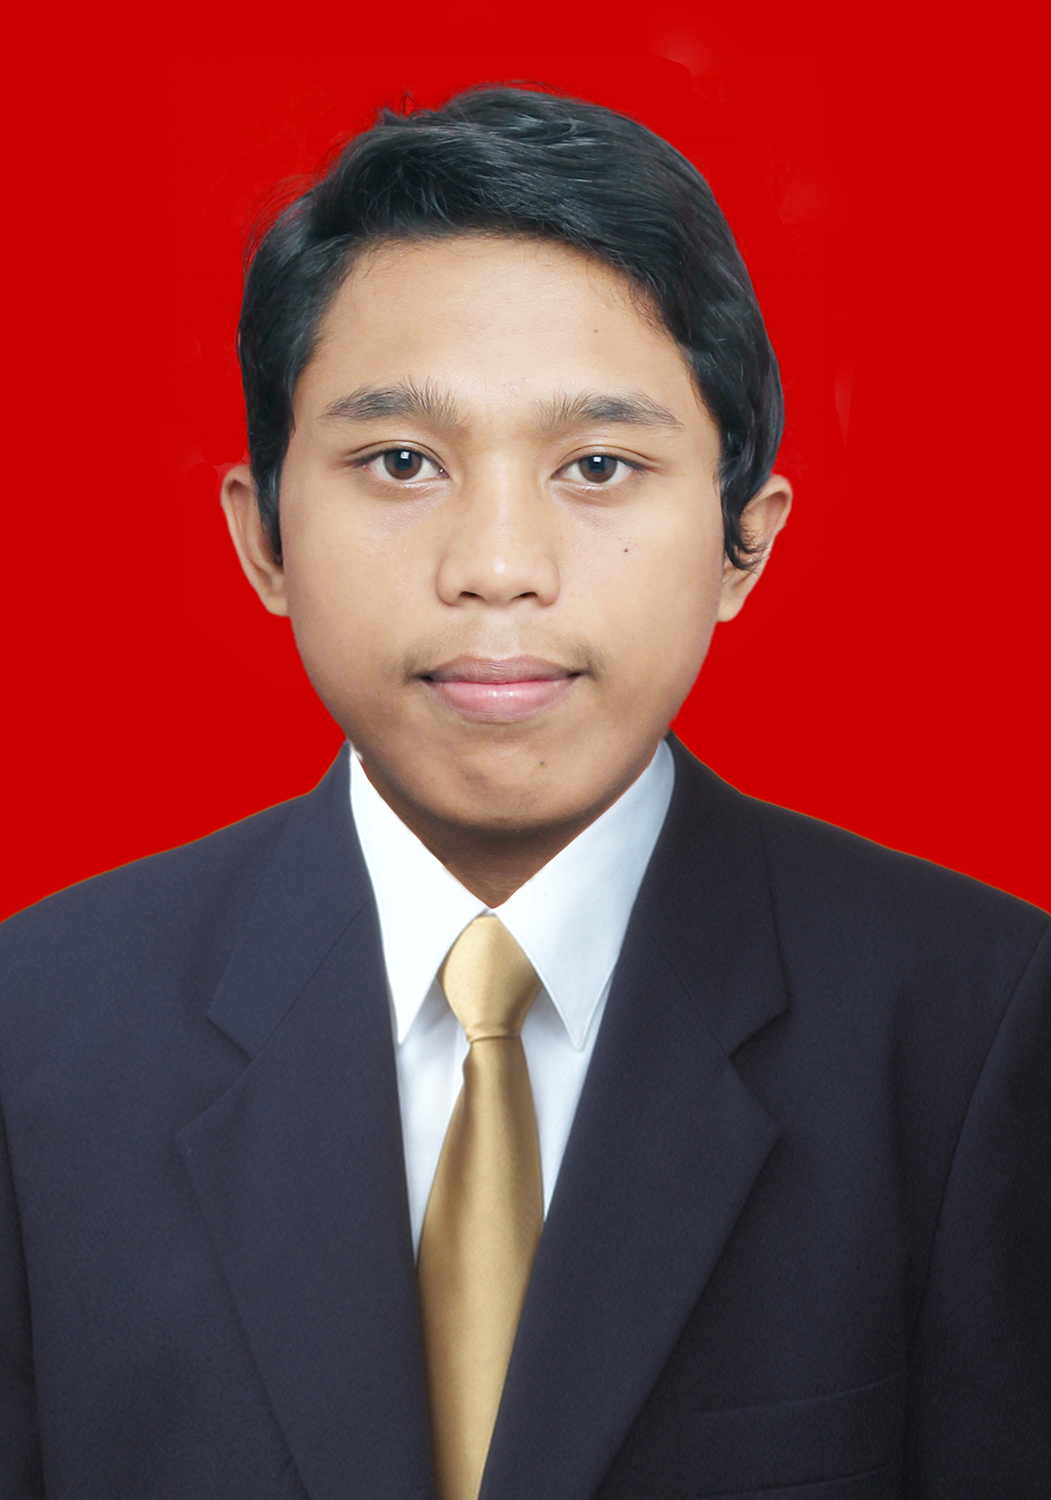
\includegraphics[width=0.45\textwidth]{foto.png}%
	\end{figure}
\end{minipage}



\hfill \break
\hfill \break

\end{document}

%%%%%%%%%%%%%%%%%%%%%%%%%% End CV Document %%%%%%%%%%%%%%%%%%%%%%%%%%%%%

%----------------------------------------------------------------------%
% The following is copyright and licensing information for
% redistribution of this LaTeX source code; it also includes a liability
% statement. If this source code is not being redistributed to others,
% it may be omitted. It has no effect on the function of the above code.
%----------------------------------------------------------------------%
% Copyright (c) 2007, 2008, 2009, 2010, 2011 by Theodore P. Pavlic
%
% Unless otherwise expressly stated, this work is licensed under the
% Creative Commons Attribution-Noncommercial 3.0 United States License. To
% view a copy of this license, visit
% http://creativecommons.org/licenses/by-nc/3.0/us/ or send a letter to
% Creative Commons, 171 Second Street, Suite 300, San Francisco,
% California, 94105, USA.
%
% THE SOFTWARE IS PROVIDED "AS IS", WITHOUT WARRANTY OF ANY KIND, EXPRESS
% OR IMPLIED, INCLUDING BUT NOT LIMITED TO THE WARRANTIES OF
% MERCHANTABILITY, FITNESS FOR A PARTICULAR PURPOSE AND NONINFRINGEMENT.
% IN NO EVENT SHALL THE AUTHORS OR COPYRIGHT HOLDERS BE LIABLE FOR ANY
% CLAIM, DAMAGES OR OTHER LIABILITY, WHETHER IN AN ACTION OF CONTRACT,
% TORT OR OTHERWISE, ARISING FROM, OUT OF OR IN CONNECTION WITH THE
% SOFTWARE OR THE USE OR OTHER DEALINGS IN THE SOFTWARE.
%----------------------------------------------------------------------%